\chapter{Metagenomics Essentials}
\pagenumbering{arabic} \setcounter{page}{4}

This section reviews the procedural steps involved in a typical metagenomics workflow. This section also covers the pre-requisites in metagenomics which one should contemplate before setting up an experiment.

\subsection{Sampling}
Ideally, the obtained samples should be symbolic of the population from which they are pooled. Similarly, the extracted genetic material from them should be suggestive of all the cells. Also, pooled samples should carry high-quality nuclear material, which decreases the signal-to-noise ratio in the downstream analysis [2]. If the target community is linked with a host organism, selective lysis must be conducted to reduce the host DNA interference [20]. To plan the number of samples required, a refraction curve is often used [2]. The rarefaction curve proposes abundance of existing species as function of inspected species [Figure \ref{fig:figure1}]. It is also desirable to look for pilot studies to determine the number of samples required from a particular habitat.

\begin{figure}
  \centering
  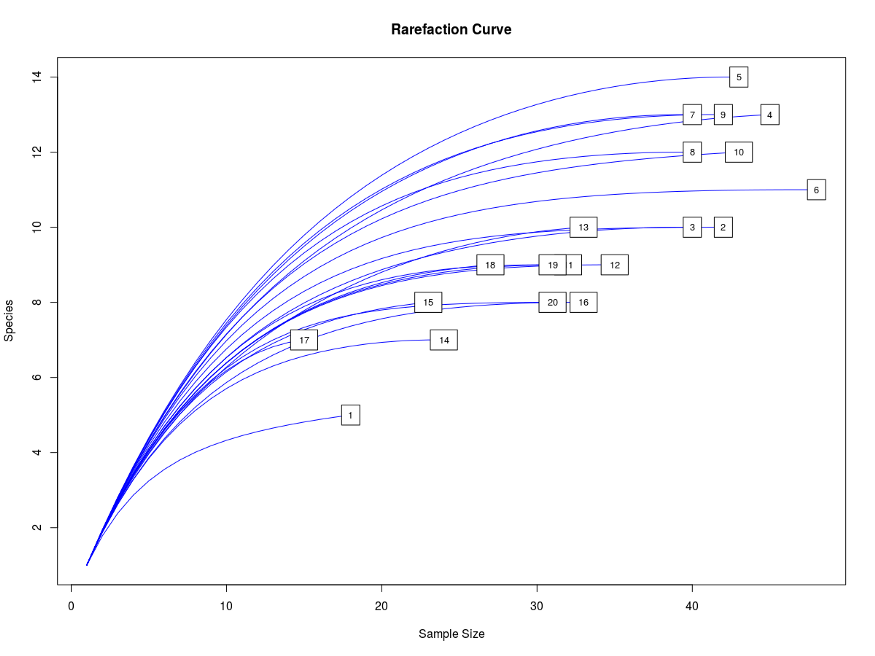
\includegraphics[width=9cm, height=5.5cm] {../figures/Figure1.png}
  \caption{Typical Rarefaction Curve, It displays how many species are identified with prolonged sampling. If sampling is ample, curves should finally plateau as it becomes tougher to find new species, despite the increase in sampling. On the other hand, if the curves are steep, more sampling is required to infer ecological judgments; Source: [21]}
  \label{fig:figure1}
\end{figure}

\subsection{Sample Quality \& Metadata}
Once the samples are secured, they should be filtered to reduce the signal to noise ratio in downstream analysis. This can be achieved by either eliminating the noise (e.g. removing virome if studying bacteria) or collecting surplus signals (e.g. collection of high-quality samples) [2]. Often it is hard to replicate metagenomic analysis as even the slightest deviation from the collection site appends variability to results. Therefore, precise documentation of the metadata is also vital to metagenomics; parameters like sampling date, time, depth, salinity, et cetera should be reported [20]. A recent report from The Genomics Standards Consortium published a standard for reporting metagenomic metadata [22].

\subsection{Sequencing}
Over the years, second-generation sequencing methods have taken over the area of genomics [Figure \ref{fig:figure2}]. The Sanger Shotgun sequencing method (SS), the reasonable option of researchers in the past, has been displaced by PCR based methods, especially for smaller metagenomes [23]. Despite being labour intensive and costly, the SS sequencing method is still fancied when dealing with specimens from low-diversity environments because it gives a comprehensive portrayal of genomes [23]. Third-generation sequencing methods are gradually becoming the preference for metagenomics as they give long reads which aid in de-novo assemblies.

\begin{figure}
  \centering
  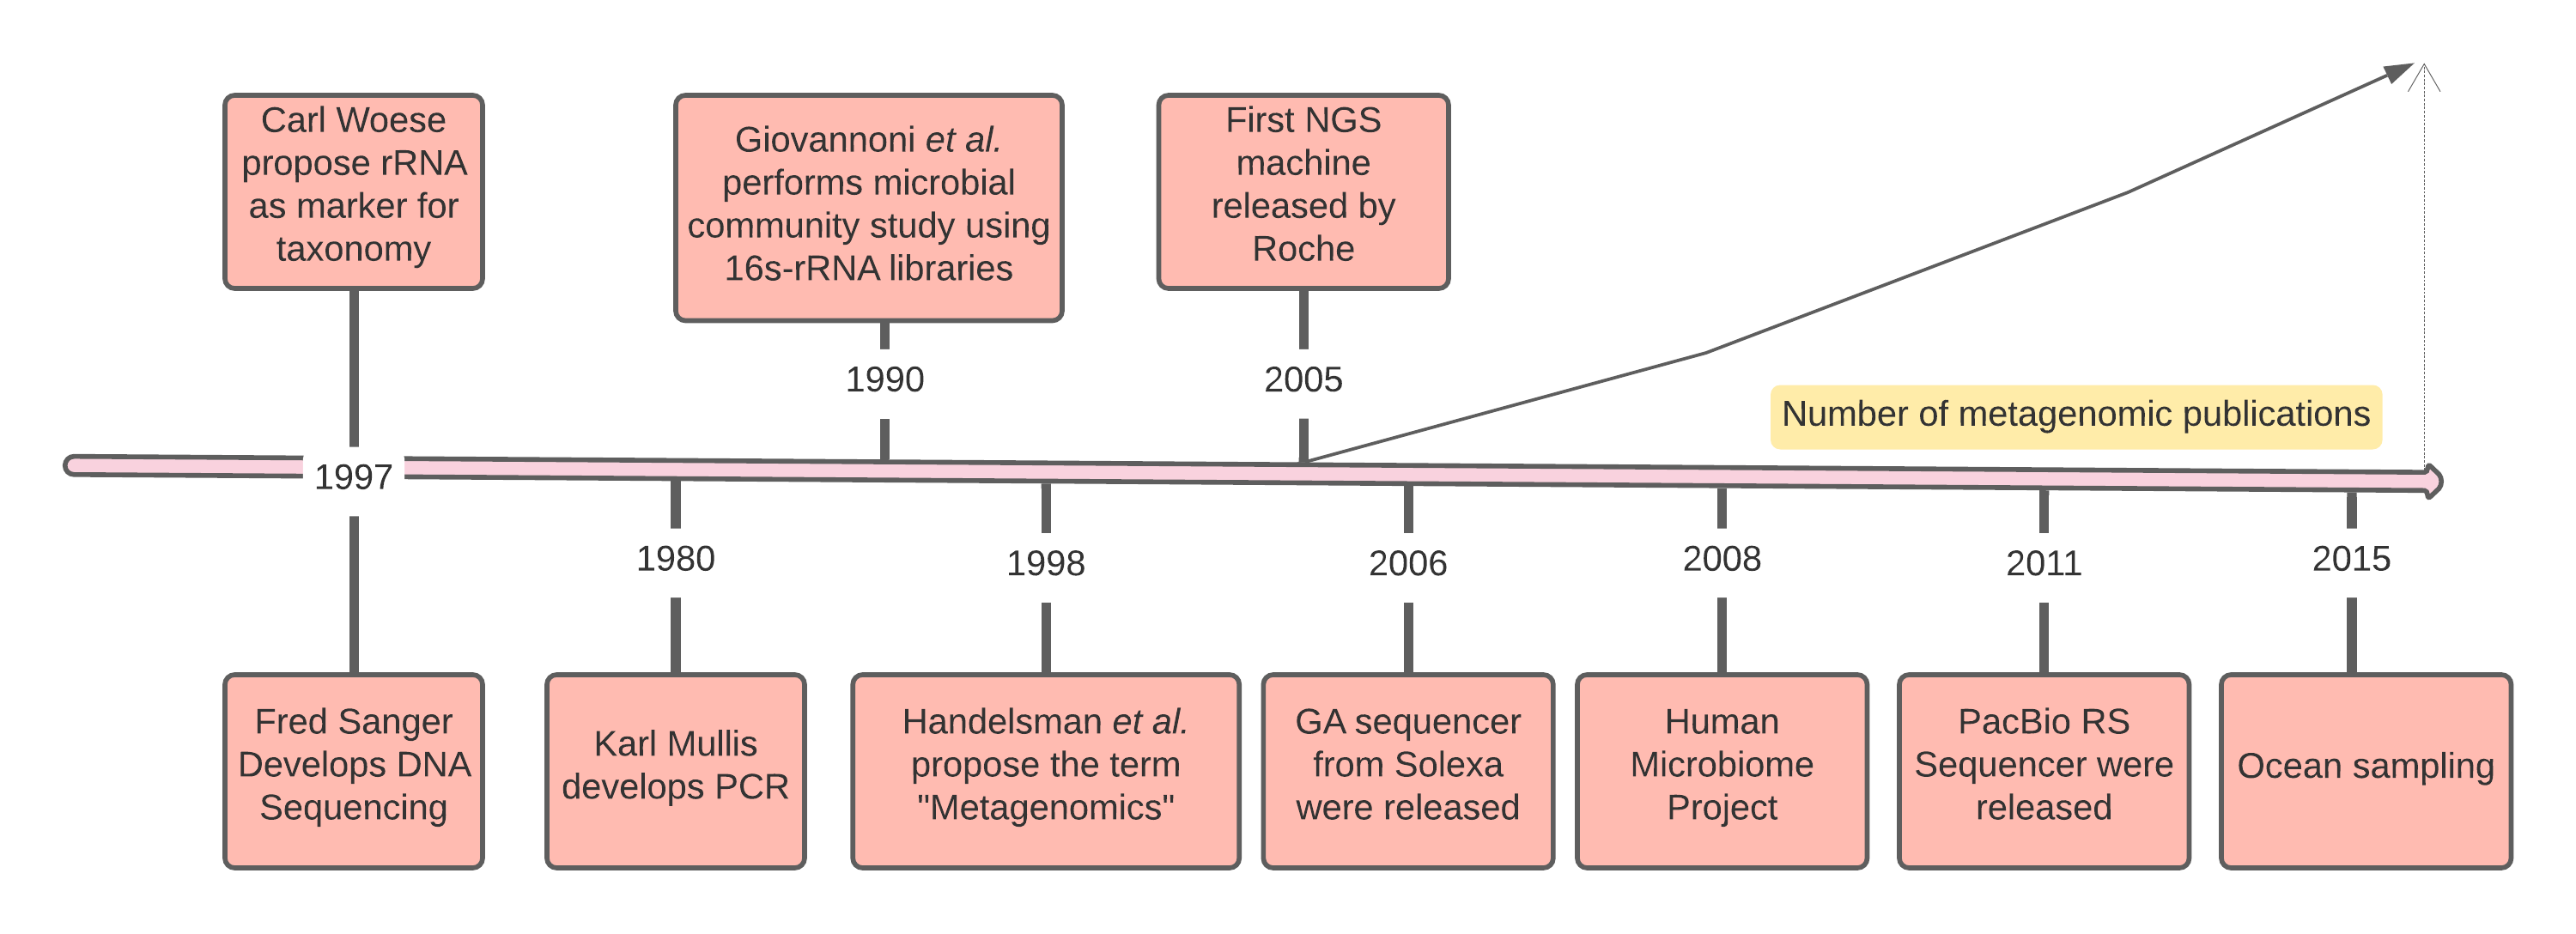
\includegraphics[width=15cm, height=6.5cm]{../figures/Figure2.png}
  \caption{Developments in Microbiology with sequencing technology, Infographic displays the rise in the number of publications about metagenomics as the successive generations of sequencers were released starting from 2005; Source: [2]}
  \label{fig:figure2}
\end{figure}

\subsection{Sequence Coverage}
Coverage is represented by the average amount of times a nucleotide gets sequenced [24]. Therefore, if there is a 10X coverage, then each nucleotide is sequenced ~ ten times. We can measure the expected number reads needed to sequence the whole genome by fitting a Poisson distribution model, which is derived through the Lander-Waterman equation as follows [24],

\begin{equation} 
  Coverage (C) = \frac{L * N}{G}
  \label{eq:eq1}
\end{equation}

where, L= read length, N = number of reads, and G = length of Genome

\begin{equation} 
  P_{0} = 1 - e^{-C} = P_{0} = 1 - e^{\frac{L * N}{G}}
  \label{eq:eq2}
\end{equation}

\begin{equation} 
  Number  of reads (N) = -\frac{\log(1-P_{0})}{L}* G
  \label{eq:eq3}
\end{equation}

For metagenomic sampling,

\begin{equation} 
  G_{m} = \sum_{i=1}^{\l} n_{i}G_{i}
  \label{eq:eq4}
\end{equation}

Where, $G_{i}$ is size of metagenome containing l genomes; $n_{i}$ is the number of copies of $G_{i}$

\subsection{Assembly}
Assembly of contigs is one of the requisite steps of any genomic data analysis. It allows the researcher to find the genomic elements such as transcription factor binding sites, open reading frames, et cetera. One can also locate notable size elements such as pathogenicity island by assembling longer reads [25]. Like any genomic analysis, the assembly for metagenomics can be done either with a reference dataset or without it (de-novo assembly). However, space-time complexity during de-novo assembly increases exponentially; therefore, specially tailored algorithms like de Bruijn are employed for the purpose. And, short-reads should be fabricated in large quantities to procure sufficient coverage [25]. Different read lengths, when assembled, can generate varying information about genetic elements at various levels of complexity [Table \ref{table1},2]. However, there exist potential challenges when dealing with the metagenomics data, as assembling reads from different OTUs could create interspecies chimaeras [23].

\begin{table}[ht]
\centering
\caption{Information carried by varying lengths of genomic fragments}
 \begin{tabular}{|c | c|} 
 \hline
 Sequence Length (bp) & Genomic Information \\ [0.5ex] 
 \hline\hline
 25 - 75 & SNPs, Short Frameshift Mutations \\ 
 \hline
 100 - 400 & Short functional signatures \\
 \hline
 500 - 1,000 & Whole domains, Single Domain Genes \\
 \hline
 1,000 - 5,000 & Short Operons, Multi-domain genes \\
 \hline
 5,000 - 10,000 & Long Operons, cis-control elements \\
 \hline
 More than 100,000 & Pathogenicity Islands, Mobile Insertion elements \\
 \hline
 More than 1,000,000 & Prokaryotic Chromosome Organisation \\
 \hline
\end{tabular}
\label{table1}
\end{table}

\subsection{Binning}
Binning refers to classifying sheared DNA sequences into taxonomic groups, which describe the individual genomes of the closely related species. Binning can be achieved using two strategies, i.e. either by Composition-based (CB) methods or by Similarity-based (SB) methods [26]. CB binning is prone to errors; as the number and relatedness of OTUs in metagenomes increases, miscalculation frequency also increases [26]. Therefore the CB method is preferred for the sequences which have no homologs. Even though the CB method does not yield fruitful results with short reads, the output can be improved by using training datasets of long fragments [27]. SB methods first find the similarities with the available/provided reference dataset to generate a tree and then generate the inferences about the sequences bins [27]. It is clearly a preferred choice of binning method for short reads as it is computationally less intensive to work with smaller contigs.

\subsection{Functional Annotation}
The functional profile of the metagenome answers vital questions about community dynamics. Ideally, the annotation shouldn't be done de-novo but using a reference dataset. Functional annotation is considerably challenging for traditional genomics data, and complexity further increases when dealing with metagenomes as the available sequences are either partial or have no homologues. The sequences which are not annotated using a reference dataset are known as ORFans and constitute a never-ending genetic recentness in metagenomics [28]. To overcome this, one can completely overlook the gene-calling steps and utilize six-frame translation on reads; if the translated frames are adequately long, then they can be considered as ORFs; which can then be used for annotating signatures (HMM profiles etc.). The motif EXtraction (MEX) program works on the same principle and can identify enzymatic elements from sequence data [29].

\subsection{Future}
Metagenomics has made novel breakthroughs over the years; it has benefited ecology and has also backed up gut microbiology. Turnbaugh et al. have published a study showing a correlation between obesity and gut-microbiome [30]. With PacBio SMRT and Oxford Nanopore's discovery, the second-generation methods will soon be replaced by long-read sequencers, which will assist de-novo assemblies and annotations [31].